\subsection{Simulation des Greifarms\hfill\textnormal{\emph{Berger}}}
writen in python 

export with \footnote{http://wiki.ros.org/sw\_urdf\_exporter}

Das Skript generiert aus den URDF-Daten eine sogenannte "Chain".
Eine zweite Funktion nimmt diese Chain und ein Array mit Koordinaten entgegen
und gibt die Ausrichtung der Kettenglieder aus.
Diese ausgerichtete Kette wird dann, 
wie in Abbildung \ref{fig:greifarm1} dargestellt,
mit dem Matplotlib-Package visualisiert werden.

\begin{figure}[H]
  \centering{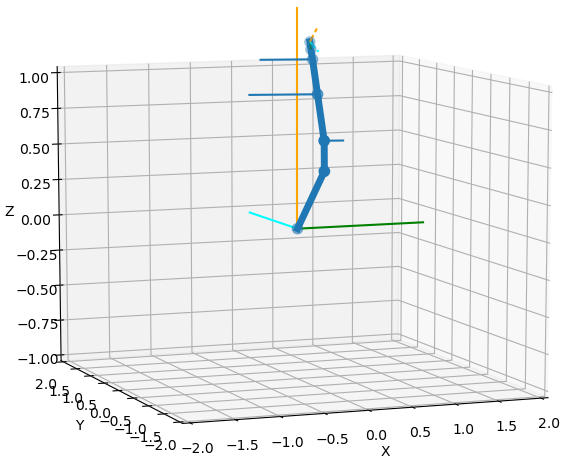
\includegraphics[width=1.0\linewidth]{Abbildungen/greifarm1.png}}
  \caption{Matplotlib ouput}
  \label{fig:greifarm1}
\end{figure}

Alternativ könnten diese Daten auch an einen tatsächlichen Roboter-Arm weitergegeben werden.
Der Rescue-Robot müsste nur die relative Position des zu greifenden Objekts berechnen
und könnte dann das Objekt greifen und dann eine Position über dem Container anfahren.
